\begin{chapter}{Come funziona}

\begin{section}{Schema generale}
ANT \`e diviso in tre componenti logici principali: il \textbf{parser}, la \textbf{
working memory} e gli \textbf{algoritmi}. Ognuno di questi tre componenti
\`e collegato agli altri secondo lo schema seguente:

\begin{figure}[!htb]
	\centering
	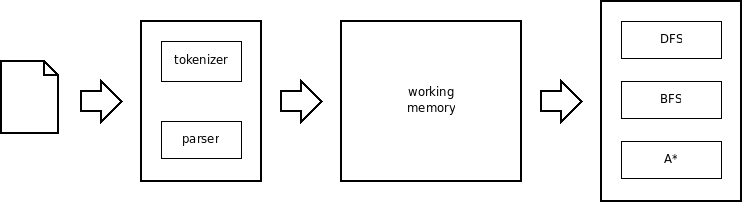
\includegraphics[scale=.45]{img/schemagenerale.png}
	\caption{Schema generale del funzionamento di ANT}
	\label{fig:schemagenerale}
\end{figure}

Si noti che il parser \`e a sua volta diviso in due componenti, il tokenizer
ed il parser vero e proprio, il cui funzionamento verr\`a illustrato in dettaglio
in \ref{sec:parsing-overview}.
La working memory \`e la componente che mantiene in memoria fatti e regole. Verr\`a
descritta in dettaglio in \ref{sec:workingmemory-overview}.
La gestione degli algoritmi verr\`a affrontata, assieme a una descrizione pi\`u
specifica del funzionamento degli stessi, nel capitolo \ref{sec:algoritmi}.

\end{section}

\begin{section}{Grammatica del linguaggio}
Un file sorgente in ANT \`e diviso in quattro componenti principali:
\begin{enumerate}
	\item il blocco delle opzioni
	\item il blocco di fatti
	\item il blocco delle regole
	\item il blocco delle euristiche (opzionale)
\end{enumerate}
\noindent La grammatica completa in notazione BNF \`e disponibile in \ref{sec:grammar}.

	\begin{subsection}{Il blocco delle opzioni}
	\label{sec:option-block}
	Il blocco delle opzioni \`e identificato dalle parole chiave \verb,set, e \verb,endSet, e deve
	essere unico all'interno di tutto il file sorgente
	Ad esempio:

	\begin{verbatim}
	set
	  opzione1 "valore1";
	  opzione2 "valore2";
	  opzione3 3;
	endSet
	\end{verbatim}

	\noindent Le opzioni disponibili sono (obbligatorie a meno che non specificato diversamente):
	\begin{itemize}
		\item \verb,algo,: imposta l'algoritmo da utilizzare per la risoluzione del problema, pu\`o
		essere uno tra \verb,bfs, per la ricerca in ampiezza, \verb,dfs, per la ricerca in profondit\`a,
		\verb,astar, per l'algoritmo A* e \verb,hill, per l'algoritmo di ricerca a salita pi\`u
		ripida (\textit{Hill Climbing})
		\item \verb,limit,: opzionale se l'algoritmo scelto \`e A*, obbligatorio per gli altri algoritmi,
		imposta il limite di profondit\`a per l'algoritmo
		\item \verb,start,: il nome del fatto iniziale
		\item \verb,stop,: il nome del fatto finale
		\item \verb,heuristic,: il nome della funzione euristica, da utilizzare solo se l'algoritmo
		scelto \`e A* oppure quello dell'Hill Climbing
	\end{itemize}
	\end{subsection}

	\begin{subsection}{Il blocco dei fatti}
	Il blocco di un fatto \`e identificato dalle keyword \verb,beginFact, e \verb,endFact,. Ad
	ogni fatto \`e associato un nome di riferimento che deve essere univoco all'interno del
	sorgente. Ogni fatto presenta una lista di attributi che possono assumere valori numerici
	o stringhe. Ad esempio:

	\begin{verbatim}
	beginFact fatto
	  attributo1 = "stringa";
	  attributo2 = 10000;
	  attributo3 = "altra stringa";
	endFact
	\end{verbatim}

	\noindent Non vengono imposti limiti\footnote{sebbene siano presenti, ovviamente, limiti pratici
    sulla quantit\`a di memoria disponibile} sul numero di attributi di un fatto.
	\end{subsection}

	\begin{subsection}{Il blocco delle regole}
	Una regola \`e identificata dalle keyword \verb,beginRule, e \verb,endRule,. Ad
	ogni regola \`e associato un nome di riferimento che deve essere univoco all'interno del
	sorgente. Ogni regola si divide in due parti: LHS (Left Hand Side), parte sinistra, e RHS
	(Right Hand Side), parte destra. Queste due parti sono separate dal carattere \verb,>,.

	La parte sinistra \`e quella che verifica l'applicabilit\`a della regola e non \`e altro
	che un espressione booleana, mentre la parte destra \`e quella che applica modifiche
	alla base di fatti. Le regole possono definire variabili che verranno risolte tramite
	il processo di matching descritto in \ref{sec:matching}. Ad esempio:

	\begin{verbatim}
	beginRule regola
	  equals("attributo", valore) and
	  gt(valore, 3)
	  >
	  remove("attributo");
	endRule
	\end{verbatim}

	\noindent Una lista dei predicati disponibili si trova in \ref{sec:predicates}.
	\end{subsection}

	\begin{subsection}{Il blocco delle euristiche}
    \label{sec:heuristic-block}
    \`E possibile definire, nel caso l'algoritmo specificato lo richieda, una o pi\`u funzioni
    euristiche all'interno di un sorgente. Le euristiche vengono identificate dalle keyword
    \verb,beginHeuristic, e \verb,endHeuristic, che servono rispettivamente a indicare l'inizio di
    una funzione euristica e la sua fine. Ad ogni euristica va associato un nome univoco
    tra le euristiche che verr\`a usato poi per indicare nell'opzione \verb,heuristic,
    (vedi la descrizione delle opzioni disponibili in \ref{sec:option-block})
    quale sar\`a l'euristica da considerare per l'algoritmo (se ha senso considerarla, infatti
    algoritmi quali il BFS e il DFS ignorano la presenza di un euristica).

    Un euristica non \`e altro che una serie di predicati per la parte destra di una regola,
    pertanto i predicati utilizzabili sono esattamente gli stessi definiti per la RHS delle 
    regole (una lista dei predicati \`e disponibile in appendice \ref{sec:predicates-rhs}).

    La vera differenza con la RHS delle regole \`e che, essendo una funzione euristica una
    funzione che ritorna un valore che rappresenta una stima della distanza dallo stato corrente
    all'obiettivo, esiste la necessit\`a di poter \textit{ritornare} il valore in questione.
    Questo viene fatto utilizzando il predicato \verb,return,, il cui unico parametro in
    input \`e il valore di ritorno dell'euristica. \`E possibile avere pi\`u \verb,return,
    all'interno della stessa euristica, ma verr\`a considerato esclusivamente l'ultimo.

    Una semplice euristica di esempio \`e quella utilizzata per il gioco dell'8, dove viene
    contato il numero di tasselli fuoriposto:

    \begin{verbatim}
	beginHeuristic tasselli_mancanti
	  define(h, 0);
	  different("cella_1_1", 1, 1, 1, res);
	  add(h, res);
	  different("cella_1_2", 1, 2, 2, res);
	  add(h, res);
	  different("cella_1_3", 1, 3, 3, res);
	  add(h, res);
	  different("cella_2_1", 2, 1, 8, res);
	  add(h, res);
	  different("cella_2_2", 2, 2, 0, res);
	  add(h, res);
	  different("cella_2_3", 2, 3, 4, res);
	  add(h, res);
	  different("cella_3_1", 3, 1, 7, res);
	  add(h, res);
	  different("cella_3_2", 3, 2, 6, res);
	  add(h, res);
	  different("cella_3_3", 3, 3, 5, res)
	  add(h, res);
	  return(h);
	endHeuristic
    \end{verbatim}

    \noindent In questa euristica, chiamata \verb,tasselli_mancanti,, viene inizializzata una
    variabile \verb,h, che \`e quella che conterr\`a il numero di tasselli fuoriposto. Per
    ogni cella del gioco, se questa non contiene il valore richiesto, viene sommato 1 ad \verb,h,.
    Alla fine \verb,h, sar\`a esattamente il valore che vogliamo far ritornare e pertanto
    procediamo con il \verb,return(h),.

	\end{subsection}

\end{section}

\begin{section}{Il parsing}
\label{sec:parsing-overview}
Il parser \`e diviso in due componenti principali, il tokenizer e il parser vero e
proprio. Il tokenizer si occupa di dividere il file sorgente in token, ovvero separa
i vari \textit{elementi} del file sorgente mentre il parser effettua controlli sulla
validit\`a della sequenza di elementi.

	\begin{subsection}{Tokenizer}
	Come gi\`a detto il tokenizer divide il sorgente in una lista di token che poi
	verranno passati al parser. \`E un automa a stati finiti che non effettua controlli
	di validit\`a semantica, ma semplicemente si assicura che ogni singolo token sia
	in una forma, ovvero di un tipo, accettabile dal programma. Per esempio, sia dato
	il seguente file sorgente:

	\begin{verbatim}
	beginFact nomefatto
	  attributo1 = "valore";
	  attributo2 = 1;
	endFact
	\end{verbatim}

	\noindent Allora verr\`a prodotta la lista seguente:

	\begin{verbatim}
	('beginFact', TKN_SYMBOL), ('nomefatto', TKN_SYMBOL),
	  ('attributo1', TKN_SYMBOL), ('=', TKN_OPERATOR),
	    ('valore', TKN_STRING), (';', TKN_OPERATOR),
	  ('attributo2', TKN_SYMBOL), ('=', TKN_OPERATOR),
	    ('1', TKN_NUMBER), (';', TKN_OPERATOR),
	('endFact', TKN_SYMBOL)
	\end{verbatim}

	\noindent Si pu\`o notare che ogni token e` una coppia valore-tipo. Il tipo pu\`o
	essere un simbolo (\verb,TKN_SYMBOL,), un operatore del linguaggio (\verb,TKN_OPERATOR,)
	o una costante (\verb,TKN_NUMBER, o \verb,TKN_STRING,). Questa lista verr\`a passata
	al parser che proceder\`a a effettuare controlli sulla semantica del sorgente.
	\end{subsection}
	
	\begin{subsection}{Parser}
	Dalla lista ricevuta dal tokenizer, il parser effettua il parsing e vero e proprio
	e inserisce le componenti riconosciute come fatti o regole all'interno delle strutture
	dati apposite. La lista di token viene inizialmente divisa in \textit{blocchi}, ognuno
	relativo ad un elemento del linguaggio come un fatto o una regola. Successivamente,
	ognuno di questi blocchi, viene diviso in sottoblocchi che vengono passati alla routine
	di parsing relativa. Ad esempio, il sorgente viene prima diviso in vari blocchi,
    ognuno specifico di un elemento del programma come il blocco delle opzioni, quello delle
    regole, dei fatti, ecc... A sua volta, ogni blocco viene diviso in sotto-blocchi, ad
    esempio un blocco di tipo fatto viene diviso in modo tale da avere una lista di coppie
    attributo-valore che verr\`a poi parsato dalla routine relativa.
	\end{subsection}
\end{section}

\begin{section}{Avviare ANT}
L'invocazione di ANT avviene tramite command line. \`E possibile passare alcune opzioni
tramite linea di comando, quali:

\begin{itemize}
	\item \verb,--input,: percorso relativo o assoluto verso il sorgente del problema da risolvere;
	\item \verb,--algo,: l'algoritmo da utilizzare. Sovrascrive l'opzione descritta in \ref{sec:option-block};
	\item \verb,--limit,: il limite da imporre sull'algoritmo (il tipo di limite dipende dall'algoritmo e
	in alcuni casi pu\`o non essere considerato). Sovrascrive l'opzione descritta in \ref{sec:option-block};
	\item \verb,--show-stats,: mostra statistiche sull'utilizzo del programma come il numero di nodi
	espansi dall'algoritmo. In ambienti UNIX-like mostra anche statistiche di utilizzo della memoria;
\end{itemize}

Per esempio, il problema dell'agricoltore risolto in \verb,esempi/agricoltore.ant,, si avvia con:

\begin{verbatim}
$ ant --input esempi/agricoltore.ant

ANT v0.77815

Facts in memory: 2
Rules in memory: 8
Processing (algorithm: bfs)...
Limit: 15
Solution found!
Sequence: 
  1. sposta_agricoltore_e_pecora_sulla_riva_lontana
  2. sposta_agricoltore_sulla_riva_vicina
  3. sposta_agricoltore_e_cavolo_sulla_riva_lontana
  4. sposta_agricoltore_e_pecora_sulla_riva_vicina
  5. sposta_agricoltore_e_lupo_sulla_riva_lontana
  6. sposta_agricoltore_sulla_riva_vicina
  7. sposta_agricoltore_e_pecora_sulla_riva_lontana
\end{verbatim}

Se volessimo usare l'algoritmo DFS senza modificare il file sorgente del problema e mostrare le
statistiche di utilizzo, potremmo invece fare:

\begin{verbatim}
$ ant --input esempi/agricoltore.ant --algo dfs --show-stats

ANT v0.77815

Facts in memory: 2
Rules in memory: 8
Processing (algorithm: dfs)...
Limit: 15
Solution found!
Sequence: 
  1. sposta_agricoltore_e_pecora_sulla_riva_lontana
  2. sposta_agricoltore_sulla_riva_vicina
  3. sposta_agricoltore_e_lupo_sulla_riva_lontana
  4. sposta_agricoltore_e_pecora_sulla_riva_vicina
  5. sposta_agricoltore_e_cavolo_sulla_riva_lontana
  6. sposta_agricoltore_sulla_riva_vicina
  7. sposta_agricoltore_e_pecora_sulla_riva_lontana
Usage statistics:
 Expanded nodes:                11
 User time used:                0,11998s
 System time used:              0,2999s
 Page reclaims:                 421
 Page faults:                   1
 No. of swaps:                  0
 Voluntary context switches:    2
 Involuntary context switches:  54
 Total memory used:             3388kB
\end{verbatim}
\end{section}

\begin{section}{La working memory}
\label{sec:workingmemory-overview}
La working memory memorizza una \textit{rappresentazione eseguibile} dei fatti e
delle regole. Sulla working memory viene eseguito il problema, ovvero viene effettuato
il matching (vedi sezione successiva, \ref{sec:matching}) sulle regole disponibili
e tali regole vengono applicate.
\end{section}

\begin{section}{Il problema del matching}
\label{sec:matching}
Il processo di ricerca delle regole applicabili per un determinato stato della working
memory \`e chiamato \textbf{matching}. In particolare, nel momento in cui abbiamo a che
fare con regole che presentano variabili al loro interno, dobbiamo \textbf{unificare}
tali regole con valori che la soddisfano, ovvero dobbiamo trovare una sostituzione delle
variabili tale che la regola risulti applicabile (questo processo \`e chiamato, appunto,
\textbf{unificazione}). Il matching \`e un processo complesso e soprattutto
computazionalmente pesante, pertanto abbiamo dovuto prendere alcuni accorgimenti in fase
di realizzazione.

Il problema \`e stato risolto nel modo seguente. Innanzitutto, le regole sono
divise in due parti logicamente distinte: la parte sinistra o \textit{Left Hand Side}
(LHS) e la parte destra o \textit{Right Hand Side} (RHS).
L'unificazione va risolta esclusivamente sulla parte sinistra; la parte destra
della regola riutilizzer\`a, se necessario, le variabili precedentemente risolte
per la LHS.

All'interno di ANT, la parte sinistra non \`e altro che un albero di espressione, ovvero
un albero binario le cui foglie sono nodi di tipo predicato, mentre le radici sono
nodi che rappresentano un espressione booleana (``and'' oppure ``or''). In questo modo
\`e possibile valutare l'albero ricorsivamente attraverso le visite canoniche quali
quelle in preordine, postordine o in ordine a seconda delle necessit\`a.

Nel caso la regola non presenti variabili, percui non sia necessario unificare, allora
viene semplicemente valutato l'albero di espressione sullo stato corrente.

L'algoritmo di unificazione implementato da ANT funziona secondo lo schema seguente.
Per ogni regola presa in esame:

\begin{enumerate}
	\item estrai una coda di predicati attraverso una visita in post-ordine
	      dell'albero di espressione
	\item dalla coda precedentemente creata, estrai una lista di variabili
	      e informazioni sul loro tipo
	\item esplora tutto lo spazio di ricerca creando un albero n-ario a partire
        dalle variabili estratte e provando, in sostanza, tutte le possibili
        combinazioni
	\item valuta la regola per ogni possibile sostituzione e aggiungi al
        conflict set solo le regole la cui LHS ritorna il valore di verit\`a "vero"
\end{enumerate}

Il cuore del problema \`e il punto tre: la creazione e gestione dell'albero pu\`o
essere un problema rilevante dato la grande quantit\`a di nodi presenti. Inizialmente
avevamo utilizzato un heap per gestire l'albero \cite{Skiena08}.
Questa scelta, fatta per ridurre il consumo di memoria essendo l'heap in sostanza un'area
contigua di memoria, \`e risultata subito inapplicabile.
Difatti, l'heap non \`e altro che un array di dimensione prefissata il cui generico
elemento alla posizione \verb,k,, in un albero \verb,n,-ario ha:

\begin{itemize}
	\item genitore in posizione $\lfloor\frac{1}{n}(k-1)\rfloor$
	\item figlio i-esimo in posizione $nk+i$, $1 \leq i \leq n$
\end{itemize}

\noindent(Nel caso di un albero binario, la formula per ottenere i figli destro e sinistro
si riduce a $2k+1$ per il figlio sinistro e $2k+2$ per il figlio destro)

La scelta dell'heap porta una serie di miglioramenti nelle prestazioni rispetto
all'utilizzo di un canonico albero n-ario con puntatori, ed \`e giustificata
dal fatto che l'albero di espressione \`e perfettamente bilanciato, pertanto
l'array non sar\`a sparso e, anzi, tutti i campi saranno utilizzati. Inoltre,
dato che i nodi sono tutti presenti in una sezione di memoria contigua (esattamente
quella occupata dall'array su cui l'heap \`e implementato), sfruttiamo la cache
del processore in due modi:

\begin{itemize}
	\item nei processori moderni la cache pu\`o variare da un minimo
          di 512k fino anche a 8Mb sui processori per server. Nel caso in cui l'albero sia
          relativamente piccolo, potremo inserirlo tutto nella cache evitando,
          quindi l'accesso alla memoria centrale con conseguente risparmio di tempo
	\item usiamo la cache line: sui moderni processori la cache line \`e una tecnica
          che ci assicura di inserire nella cache, nel momento in cui richiediamo l'accesso
          ad un dato indirizzo di memoria, un intero blocco di memoria contenente
          l'indirizzo richiesto. Questo blocco ha dimensione fissa, appunto la
          \textit{cache line} che ha grandezza variabile a seconda delle implementazioni.
          Nei processori comuni la cache line \`e grande 64 bytes ma in realt\`a
          pu\`o variare da un minimo di 8 a un massimo di 512 bytes a seconda dell'architettura
          del processore.
\end{itemize}

Come gi\`a detto, l'heap \`e risultato tuttavia inapplicabile. La motivazione risiede
nel fatto che il numero di nodi, che \`e noto a priori, \`e estremamente elevato. Inoltre,
l'heap richiede che la memoria allocata sia contigua e sia disponibile un accesso diretto
(percui la scelta dell'array). Questo ci permette di ridurre la memoria usata dai puntatori,
ma in compenso abbiamo bisogno di allocare in blocco tutta la memoria richiesta.
Consideriamo, ad esempio, il caso in cui abbiamo cinque variabili che possono assumere venti
valori. Il nostro albero sar\`a quindi un albero di grado venti e di profondit\`a cinque.
Supponiamo che ogni nodo occupi 10 bytes, allora, essendo l'albero bilanciato (ma
utilizzando un heap anche se non utilizziamo alcuni nodi questi vanno comunque allocati),
avremo bisogno di $\sum_{i=1}^5{(20^i \cdot 10)} = 67368200$ bytes, ovvero circa 65Mb.

\`E facile capire come al crescere del numero delle variabili e all'aumentare dei valori che
queste possono assumere, l'heap raggiunge presto una dimensione eccessiva. Abbiamo, quindi,
dovuto trovare una soluzione alternativa che ci permettesse comunque di risolvere velocemente,
per quanto possibile, il problema dell'unificazione. Alla fine, la scelta \`e ricaduta
su due \textit{semplici} vettori di elementi. Infatti, si pu\`o notare un pattern all'interno
di questo processo. Ovvero, una volta calcolati, i valori che le variabili possono assumere
sono sempre gli stessi indipendentemente dalla profondit\`a dell'albero (e, quindi, dalla
variabile che stiamo considerando).

Si considerano due vettori: uno terr\`a in memoria i valori che le variabili possono assumere
(chiameremo questo vettore \verb,VALUES, in seguito), l'altro invece sar\`a un vettore di
tanti elementi quanti sono le variabili (questo vettore lo chiameremo \verb,VAR,).
\verb,VAR, non fa altro che tenere in memoria a quale indice la variabile di posizione \verb,x,
punta su \verb,VALUES,. Inizialmente tutti gli elementi di \verb,VALUES, puntano al primo
elemento di \verb,VAR,. Viene quindi valutata l'espressione, con le variabili risolte
secondo l'elemento a cui esse puntano su \verb,VALUES, e in caso di successo la sostituzione
effettuata, assieme alla regola a cui essa \`e associata, viene aggiunta al conflict set.
Si incrementa quindi il valore dell'ultimo elemento di \verb,VAR, e si ripete la procedura
di valutazione. Quando questo valore raggiunge la dimensione di \verb,VALUES,, questo
viene riportato a zero e viene incrementato l'indice a cui punta la variabile seguente.
In questo modo abbiamo comunque esplorato tutto lo spazio di ricerca, ma abbiamo utilizzato
pochissima memoria rispetto all'heap. Difatti, se supponiamo che dieci variabili possono
assumere 30 possibili valori, avremo soltanto due vettori rispettivamente da 10 e 30 elementi.

\noindent Prendiamo in esame la regola che segue per capire meglio come viene
risolto il processo di unificazione:

\begin{verbatim}
beginRule
  equals(attributo1, attributo2) and
  gt(attributo2, 3)
  >
  ...
endRule
\end{verbatim}

Espressa in linguaggio naturale, la regola verr\`a soddisfatta quando ``esistono due
attributi all'interno del fatto, percui uno sia maggiore di tre e l'altro sia uguale
al primo (pertanto, anch'esso sar\`a maggiore di tre)''. Notiamo che, implicitamente,
si \`e applicato un meccanismo di inferenza sulla regola. Questo \`e un comportamento
classico nei sistemi di questo tipo.

\begin{figure}[!htb]
	\centering
	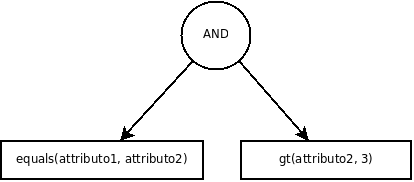
\includegraphics[scale=.45]{img/alberoregolasemplice.png}
	\caption{Albero di espressione per una regola semplice}
	\label{fig:alberoregolasemplice}
\end{figure}

Una volta costruito l'albero, ha luogo il processo di unificazione. Innanzitutto,
viene estratta dal fatto in esame una lista di attributi-valore e, successivamente,
viene creato un secondo albero (in ANT \`e implementato tramite i due vettori descritti
sopra) come in figura \ref{fig:alberounificazione}.

\begin{figure}
	\centering
	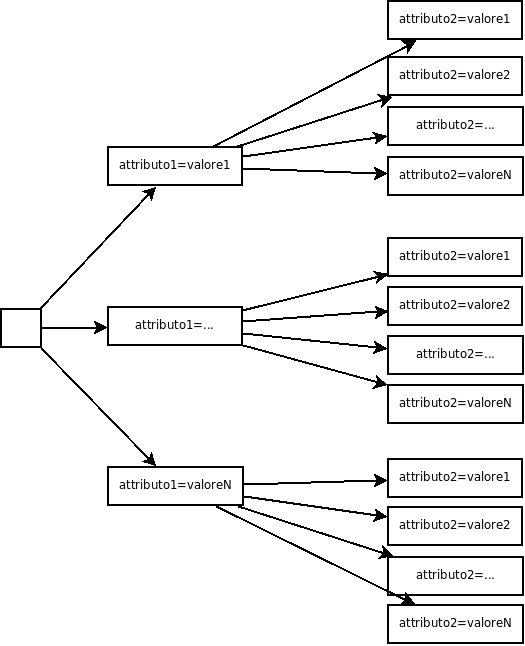
\includegraphics[scale=.45]{img/alberounificazione.png}
	\caption{Albero di unificazione}
	\label{fig:alberounificazione}
\end{figure}

Come si pu\`o notare, ogni variabile presente nella regola in esame viene
``sostituita'' con un possibile valore all'interno degli attributi del
fatto. La valutazione dell'espressione viene effettuata nel momento in si
\`e raggiunta una foglia dell'albero, e le variabili vengono sostituite
con i valori precedentemente ritrovati. Se la valutazione \`e positiva,
ovvero la regola \`e applicabile, allora tale regola assieme alle
corrispondenze variabili-valori trovate, viene aggiunta al conflict set.

Si noti che per una stessa regola possono esserci pi\`u sostituzioni valide.
Per esempio, consideriamo la seguente situazione:

\begin{verbatim}
beginFact fatto
  a = 1;
  b = 2;
  c = 3;
endFact

beginRule regola
  gte(attributo, 1)
  >
  ...
endRule
\end{verbatim}

In questo caso la regola potr\`a attivarsi tre volte con tre con differenti
sostituzioni, ovvero \verb,<attributo=1>,, \verb,<attributo=2>,, \verb,<attributo=3>,,
percui al conflict set verranno aggiunte tre diverse attivazioni che condividono la
struttura della regola ma non i valori su cui essa si applica.
\end{section}

\begin{section}{Applicazione dell'algoritmo scelto}
Indipendentemente dall'algoritmo specificato tramite l'opzione \verb,algo, oppure
quello richiesto dall'opzione \verb,--algo, per la command line, si procede in modo
simile per tutti gli algoritmi. \`E difatti possibile definire un nuovo algoritmo
senza grossi problemi, quello che \`e richiesto \`e che la funzione da richiamare
abbia la seguente firma:

\begin{verbatim}
uint32_t(*AlgoRunner)(RuleSet *ruleset,
                      Fact *initial,
                      Fact *final,
                      Options *options)
\end{verbatim}

\noindent (Il tipo di dati \verb,uint32_t, definisce un intero senza segno di 32 bit,
rimanendo per\`o indipendente dall'architettura sottostante. Questo permette di
garantire che gli interi abbiano sempre 32 bit indipendentemente dall'architettura
utilizzata, che sia x86 o ARM o Z80)\\

\noindent Ovvero, dev'essere una funzione che prende come parametri di input
un \verb,ruleset, ovvero la lista di tutte le regole presenti nel programma,
la coppia di fatti \verb,initial, e \verb,final, che rappresentano rispettivamente il
fatto da cui si parte per la computazione e il fatto a cui vogliamo arrivare ed una
lista di opzioni, ovvero tutte le opzioni definite sia tramite il blocco delle
opzioni che tramite command line (\`e sostanzialmente un dizionario le cui chiavi
sono i valori delle opzioni descritte in \ref{sec:option-block}).
\end{section}

\end{chapter}
